% !TEX root = main.tex
\documentclass[12pt,a4paper]{scrartcl}

\usepackage[latin1]{inputenc}
\usepackage{nameref}
\usepackage[colorlinks=true, urlcolor=blue, citecolor=blue, linkcolor=blue]{hyperref}
\usepackage{amsfonts, amsmath, amssymb, amsthm, thmtools}
\usepackage{cleveref}

\declaretheorem[name=Theorem, refname={Theorem, Theorems}, Refname={Theorem, Theorems}, parent=section]{theorem}
\declaretheorem[name=Corollary, refname={corollary, corollaries}, Refname={Corollary, Corollaries}, sibling=theorem]{corollary}
\declaretheorem[name=Definition, refname={definition, definitions}, Refname={Definition, Definition}, sibling=theorem, style=definition]{definition}
\declaretheorem[name=Example, refname={example, examples}, Refname={Examples, Examples}, sibling=theorem, style=definition]{example}
\declaretheorem[name=Lemma, refname={lemma, lemmas}, Refname={Lemma, Lemmas}, sibling=theorem]{lemma}
\declaretheorem[name=Exercise, refname={exercise, exercises}, Refname={Exercise, Exercises}, sibling=theorem, style=definition]{exercise}
\declaretheorem[name=Remark, refname={remark, remarks}, Refname={Remark, Remarks}, sibling=theorem, style=definition]{remark}

%\newcommand{\crefpairconjunction}{ and }
%\newcommand{\crefmiddleconjunction}{hconjunctioni}
%\newcommand{\creflastconjunction}{ and }

\usepackage{color, enumitem, fancyhdr, float, layout, multirow, setspace, verbatim}
\usepackage{algorithm2e, algorithmicx, listings}
\usepackage{caption, subcaption}
\usepackage[authoryear]{natbib}
\usepackage[all]{xy}
\usepackage{authblk}
\usepackage{leftindex}
\usepackage{tikz}
\bibpunct[; ]{(}{)}{,}{a}{,}{;}


\usepackage{graphicx}
\graphicspath{{figures/}{../figures/}}
\usepackage[authoryear]{natbib}

\textheight25cm \footskip0.5cm \topmargin-1.5cm \headsep0.2cm
\oddsidemargin-1.5cm \evensidemargin-1.5cm
\marginparwidth0cm \marginparsep = 0pt
\textwidth19cm
\doublespacing

\def\half{\frac{1}{2}}
\def\Re{\mathbb{R}}

\def\E{\mathbb{E}}
\def\F{\mathbb{F}}
\def\G{\mathbb{G}}
\def\I{\mathbb{I}}
\def\N{\mathbb{N}}
\def\P{\mathbb{P}}
\def\U{\mathbb{U}}
\def\Z{\mathbb{Z}}

\def\AA{\square}
\def\II{\Diamond}
\def\RR{\lnot \Diamond}
\def\UU{\nabla}

\def\DD{\mathcal{D}}
\def\FF{\mathcal{F}}
\def\GG{\mathcal{G}}
\def\LL{\mathcal{L}}
\def\PP{\mathcal{P}}

\def\sX{\mathcal{X}}

\def\half{\frac{1}{2}}
\def\btheta{\boldsymbol{\theta}}
\def\a{{\vec{a}}}
\def\cc{{\vec{c}}}
\def\I{{\mathbb I}}
\def\p{{\vec{p}}}
\def\w{{\vec{w}}}
\def\x{{x}}
\def\mX{{\mathbb{X}}}
\def\X{{\vec{X}}}
\def\Y{{\vec{Y}}}
\def\y{{\vec{y}}}
\def\K{{\vec{K}}}
\def\E{{\textbf{E}}}
\def\EX{{\mathbb E}}
\def\P{{\mathbb P}}
\def\V{{\mathbb V}}
\def\Re{{\mathbb R}}
\def\hE{{{\hat{\E}}}}
\def\sD{\mathcal{D}}
\def\sE{\mathcal{E}}
\def\sH{\mathcal{H}}
\def\sL{\mathcal{L}}
\def\sP{\mathcal{P}}
\def\sU{\mathcal{U}}
\def\sX{\mathcal{X}}
\def\Beps{{\boldsymbol{\epsilon}}}
\def\Bbeta{{\boldsymbol{\beta}}}
\def\Bgamma{{\boldsymbol{\gamma}}}
\def\t0{{\theta_0}}
\def\ts{{\theta^*}}
\def\tso{{\theta^*_1}}
\def\tst{{\theta^*_2}}
\def\fs{{\phi^*}}
\def\to{{\theta_1}}
\def\ts{{\theta^*}}
\def\tz{{\theta_0}}
\def\Tz{{\Theta_0}}
\def\Tzc{{\Theta_0^c}}

\def\phix{{\phi,x}} 
\def\hth{{ \hat{\theta} }}

\def\probsumm{{probability summary}}
\def\summ{{summary}}
\def\summs{{summaries}}
\def\stdsumm{{binary summary}}
\def\stdsumms{{binary summaries}}
\def\Stdsumms{{Binary summaries}}

\newcommand{\red}[1]{\textbf{\color{red}(#1)}}

\newcommand{\gfbstfig}{
 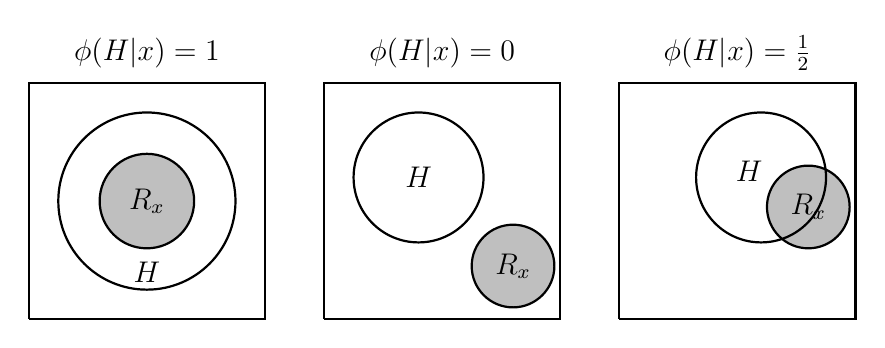
\begin{tikzpicture}[thick,scale=0.75, every node/.style={scale=0.9}]
  \draw (-6,2) circle (1.5);
  \draw [fill=lightgray] (-6,2) circle (0.8);
  \draw (-8,0) -- (-4,0) -- (-4,4) -- (-8,4) -- (-8,0);
  \node at (-6,2) {{\large $R_x$}}; 
  \node at (-6,0.8) {{\large $H$}};
  \node at (-6,4.5) {{\large $\phi(H|x) = 1$}};
			
  \draw (-1.4,2.4) circle (1.1);
  \draw [fill=lightgray] (0.2,0.9) circle (0.7);
  \draw (-3,0) -- (1,0) -- (1,4) -- (-3,4) -- (-3,0);
  \node at (0.2,0.9) {{\large$R_x$}}; 
  \node at (-1.4,2.4) {{\large $H$}};
  \node at (-1,4.5) {{\large $\phi(H|x) = 0$}};	
			
  \draw [fill=lightgray] (5.2,1.9) circle (0.7); 
  \draw (4.4,2.4) circle (1.1);
  \draw (2,0) -- (6,0) -- (6,4) -- (2,4) -- (2,0);
  \node at (5.2,1.9) {{\large $R_x$}}; 
  \node at (4.2,2.5) {{\large $H$}};
  \node at (4,4.5) {{\large $\phi(H|x) = \half$}};	
 \end{tikzpicture}
}



\title{The coherence of logical coherence}
\author{}
\date{\today}